\documentclass{beamer}
\usepackage{bookmark}
\usepackage[T5]{fontenc}
\usepackage[utf8]{vietnam}
\usepackage{lmodern} % Fix font shape warning
\usepackage{amsmath}
\usepackage{tikz}
\usetikzlibrary{positioning,arrows.meta}
\usepackage{tcolorbox}
\usepackage{graphicx}
\usetheme{Madrid}

% --- Định nghĩa màu sắc ---
\definecolor{mainblue}{RGB}{0, 32, 96}
\definecolor{footgray}{RGB}{108,113,197}
\definecolor{footred}{RGB}{255,50,50}
\definecolor{mainred}{RGB}{220,20,60} % Màu đỏ cho nút được chọn

% --- Cấu hình Footer (Bo tròn & Thông tin động) ---a
\setbeamertemplate{footline}{
  \leavevmode%
  \hbox{%
    \begin{tcolorbox}[colback=footgray, colframe=footgray, sharp corners=south, rounded corners=north, size=small, width=.3333\paperwidth, height=1.2em, halign=center, valign=center, coltext=white, boxrule=0pt]
        \tiny Phần \insertsectionnumber
    \end{tcolorbox}%
    \begin{tcolorbox}[colback=mainblue, colframe=mainblue, sharp corners=south, rounded corners=north, size=small, width=.3333\paperwidth, height=1.2em, halign=center, valign=center, coltext=white, boxrule=0pt]
        \tiny \insertsection
    \end{tcolorbox}%
    \begin{tcolorbox}[colback=footred, colframe=footred, sharp corners=south, rounded corners=north, size=small, width=.3333\paperwidth, height=1.2em, halign=center, valign=center, coltext=white, boxrule=0pt]
        \tiny Trang \insertframenumber/\inserttotalframenumber
    \end{tcolorbox}%
  }%
  \vskip0pt%
}

% Bỏ các navigation symbols thừa
\setbeamertemplate{navigation symbols}{}

\begin{document}

% --- Trang tiêu đề ---
{
\usebackgroundtemplate{

\includegraphics[width=\paperwidth,height=\paperheight]{vanh.jpg}
}

\begin{frame}
\vspace{4cm}
\centering

\vspace{1.5cm}

\begin{tcolorbox}[
colback=white,
colframe=mainblue,
width=1\textwidth,
arc=10pt,
boxrule=2pt
]

\centering
\Huge \textbf{LÝ THUYẾT ĐỒ THỊ}

\vspace{0.4cm}

\Large knguyen -- vhung -- vanh

\end{tcolorbox}

\end{frame}
}
%=================

% --- Phần 1 ---
\section{Mở đầu}
\begin{frame}{Đồ thị là gì?}
Đồ thị là cấu trúc toán học gồm:
\[ G = (V,E) \]
\begin{itemize}
\item $V$ : tập các đỉnh
\item $E$ : tập các cạnh nối các đỉnh
\end{itemize}
\end{frame}
%=================

% --- Phần 2 ---
\begin{frame}{Google Maps – Tìm đường đi ngắn nhất}

\begin{columns}

%================ LEFT =================
\column{0.55\textwidth}

\begin{tcolorbox}[colback=blue!5,colframe=mainblue,title=Bài toán]
Tìm đường đi ngắn nhất từ \textbf{A} đến \textbf{B}
\end{tcolorbox}

\vspace{0.3cm}

\begin{itemize}
\item Các giao lộ $\rightarrow$ \textbf{Đỉnh (Vertices)}
\item Các con đường $\rightarrow$ \textbf{Cạnh (Edges)}
\item Thời gian / Khoảng cách $\rightarrow$ \textbf{Trọng số}
\end{itemize}

\vspace{0.2cm}

\begin{tcolorbox}[colback=green!5,colframe=green!50!black,title=Thuật toán gợi ý của Hưng:]
Sử dụng \textbf{Dijkstra} để tìm đường đi ngắn nhất
\end{tcolorbox}

%================ RIGHT =================
\column{0.45\textwidth}

\centering
\begin{tikzpicture}[node distance=2cm, scale=0.9, every node/.style={transform shape}]

% Nodes
\node[node_base, fill=red!60] (A) {A};
\node[node_base, above right of=A] (X) {X};
\node[node_base, right of=X] (Z) {Z};
\node[node_base, below right of=A] (Y) {Y};
\node[node_base, right of=Y, fill=green!60] (B) {B};

% Edges
\draw[-, thick] (A) -- node[above] {5} (X);
\draw[-, thick] (X) -- node[above] {2} (Z);
\draw[-, thick] (A) -- node[below] {3} (Y);
\draw[-, thick] (Y) -- node[below] {6} (B);
\draw[-, thick] (Z) -- node[right] {3} (B);
\draw[-, thick] (Y) -- node[right] {4} (Z);

% Shortest path highlight
\draw[->, very thick, green!60!black] (A) -- (Y);
\draw[->, very thick, green!60!black] (Y) -- (Z);
\draw[->, very thick, green!60!black] (Z) -- (B);

\end{tikzpicture}

\end{columns}

\end{frame}
%=================

% --- Phần 3 ---
\section{Khái niệm cơ bản}
\begin{frame}{Ví dụ đồ thị}
\centering
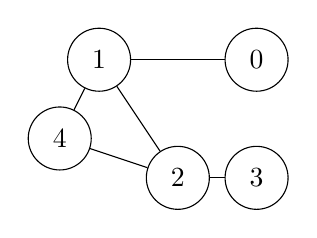
\begin{tikzpicture}[every node/.style={circle,draw,minimum size=8mm}]
\node (1) at (0,1) {1};
\node (2) at (1,-0.5) {2};
\node (3) at (2,-0.5) {3};
\node (4) at (-0.5,0) {4};
\node (0) at (2,1) {0};
\draw (1)--(4); \draw (1)--(0); \draw (1)--(2); \draw (2)--(3); \draw (4)--(2);
\end{tikzpicture}
\end{frame}
%==============

% --- Phần 4 ----
\begin{frame}{Thành phần của đồ thị}
\begin{itemize}

\item Đỉnh (Vertices)

\item Cạnh (Edges)

\item Bậc của đỉnh

\item Đường đi (Path)

\end{itemize}

\end{frame}
%=======================

% --- Phần 5 ---
\begin{frame}{Thành phần của đồ thị}

\begin{center} 
\textbf{VÍ DỤ VỀ ĐƯỜNG ĐI CỦA MỘT ĐỒ THỊ}
\end{center}

\end{frame}
%=======================

% --- Phần 3: Đường đi ---
\section{Đường đi}
\begin{frame}{Bước 1: Bắt đầu}
\centering
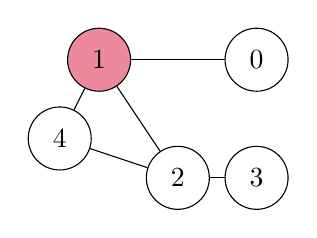
\begin{tikzpicture}[every node/.style={circle,draw,minimum size=8mm}]
\node[fill=mainred!50] (1) at (0,1) {1};
\node (2) at (1,-0.5) {2};
\node (3) at (2,-0.5) {3};
\node (4) at (-0.5,0) {4};
\node (0) at (2,1) {0};
\draw (1)--(4); \draw (1)--(0); \draw (1)--(2); \draw (2)--(3); \draw (4)--(2);
\end{tikzpicture}
\end{frame}

\begin{frame}{Bước 2: Di chuyển đến đỉnh 4}
\centering
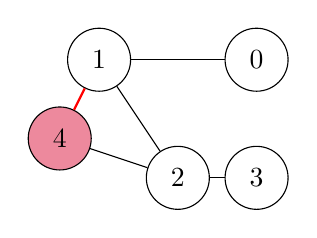
\begin{tikzpicture}[every node/.style={circle,draw,minimum size=8mm}]
\node (1) at (0,1) {1};
\node (2) at (1,-0.5) {2};
\node (3) at (2,-0.5) {3};
\node[fill=mainred!50] (4) at (-0.5,0) {4};
\node (0) at (2,1) {0};
\draw[red,thick] (1)--(4); \draw (1)--(0); \draw (1)--(2); \draw (2)--(3); \draw (4)--(2);
\end{tikzpicture}
\end{frame}

\begin{frame}{Bước 3: Di chuyển đến đỉnh 2}
\centering
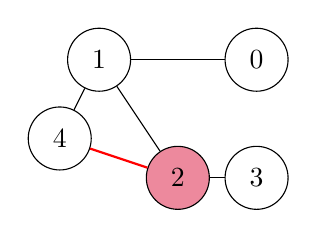
\begin{tikzpicture}[every node/.style={circle,draw,minimum size=8mm}]
\node (1) at (0,1) {1};
\node[fill=mainred!50] (2) at (1,-0.5) {2};
\node (3) at (2,-0.5) {3};
\node (4) at (-0.5,0) {4};
\node (0) at (2,1) {0};
\draw (1)--(4); \draw (1)--(0); \draw (1)--(2); \draw[red,thick] (4)--(2); \draw (2)--(3);
\end{tikzpicture}
\end{frame}

\begin{frame}{Bước 4: Di chuyển đến đỉnh 3}
\centering
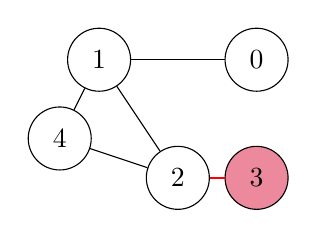
\begin{tikzpicture}[every node/.style={circle,draw,minimum size=8mm}]
\node (1) at (0,1) {1};
\node (2) at (1,-0.5) {2};
\node[fill=mainred!50] (3) at (2,-0.5) {3};
\node (4) at (-0.5,0) {4};
\node (0) at (2,1) {0};
\draw (1)--(4); \draw (1)--(0); \draw (1)--(2); \draw (4)--(2); \draw[red,thick] (2)--(3);
\end{tikzpicture}
\end{frame}

%==================

\section{Cài đặt C++}
\begin{frame}{Biểu diễn: Danh sách kề (Adjacency List)}
    \begin{columns}
        \begin{column}{0.45\textwidth}
            \textbf{Cấu trúc:}
            Mỗi đỉnh lưu một danh sách các đỉnh láng giềng.
            \vspace{0.3cm}
            \begin{itemize}
                \item \textbf{Đỉnh 1:} [4, 0, 2]
                \item \textbf{Đỉnh 2:} [1, 3, 4]
                \item \textbf{Đỉnh 3:} [2]
            \end{itemize}
        \end{column}
        \begin{column}{0.5\textwidth}
            \textbf{Ưu điểm:}
            \begin{itemize}
                \item \textbf{Tiết kiệm bộ nhớ:} Chỉ tốn $O(V+E)$.
                \item \textbf{Duyệt nhanh:} Duyệt các đỉnh kề mất $O(deg(u))$.
                \item Phù hợp cho đồ thị lớn, đồ thị thưa.
            \end{itemize}
        \end{column}
    \end{columns}
\end{frame}
\begin{frame}[fragile]{Biểu diễn: Danh sách kề}
Danh sách kề sử dụng mảng vector để lưu trữ các đỉnh láng giềng.
\begin{verbatim}
int main() {
    int n, m; // số đỉnh, số cạnh
    cin >> n >> m;
    for(int i=0; i<m; i++){
        int u, v; cin >> u >> v;
        adj[u].push_back(v);
        adj[v].push_back(u); // Đồ thị vô hướng
    }
    return 0;
}
\end{verbatim}
\end{frame}
%----------------

\begin{frame}{Biểu diễn: Danh sách cạnh (Edge List)}
\begin{itemize}
    \item Lưu trữ danh sách các cặp đỉnh $(u, v)$ tạo thành cạnh.
    \item Rất hiệu quả khi thuật toán chỉ cần duyệt qua từng cạnh một.\\
    \textbf{Đặc điểm:}
    \begin{itemize}
        \item Dễ cài đặt, tốn ít bộ nhớ.
        \item Phù hợp với các thuật toán chỉ quan tâm đến các cạnh (như Kruskal, Bellman-Ford).
        \item Không hiệu quả khi cần tìm các đỉnh kề của một đỉnh cụ thể.
    \end{itemize}
\end{itemize}
\vspace{0.5cm}
\centering
\textbf{Ví dụ:}
\begin{table}[]
    \centering
    \begin{tabular}{|c|c|c|}
        \hline
        \textbf{STT} & \textbf{Đỉnh u} & \textbf{Đỉnh v} \\ \hline
        1 & 1 & 4 \\ \hline
        2 & 1 & 0 \\ \hline
        3 & 1 & 2 \\ \hline
        4 & 2 & 3 \\ \hline
        5 & 4 & 2 \\ \hline
    \end{tabular}
\end{table}
\end{frame}

\begin{frame}[fragile]{Biểu diễn: Danh sách cạnh}
    Danh sách cạnh lưu trữ đồ thị dưới dạng tập hợp các cặp đỉnh.
    \begin{verbatim}
struct Edge {
    int u, v;
};
vector<Edge> edgeList;

// Thêm cạnh
edgeList.push_back({u, v});
    \end{verbatim}
\end{frame}

%=============
\begin{frame}{Biểu diễn: Ma trận kề (Adjacency Matrix)}
    \begin{columns}
        \begin{column}{0.4\textwidth}
            Ma trận $A$ kích thước $N \times N$:
            \begin{itemize}
                \item $A[i][j] = 1$: Nếu có cạnh nối $i$ và $j$.
                \item $A[i][j] = 0$: Nếu không có.
            \end{itemize}
        \end{column}
        \begin{column}{0.6\textwidth}
            \centering
            Đồ thị 3 đỉnh:
            \[
            A = \begin{pmatrix} 0 & 1 & 0 \\ 1 & 0 & 1 \\ 0 & 1 & 0 \end{pmatrix}
            \]
            \small (Dòng 1 nối với đỉnh 2, Dòng 2 nối 1 và 3, v.v.)
        \end{column}
    \end{columns}
    \textbf{Nhược điểm:} Tốn bộ nhớ $O(N^2)$, không tối ưu với đồ thị có hàng chục ngàn đỉnh.
\end{frame}

\begin{frame}[fragile]{Biểu diễn: Ma trận kề}
    \begin{verbatim}
// Ma trận kích thước tối đa 100x100
int adj[100][100]; 
int main() {
    int n, m; // số đỉnh, số cạnh
    cin >> n >> m;
    
    for(int i = 0; i < m; i++) {
        int u, v; cin >> u >> v;
        // Đồ thị vô hướng: đánh dấu 1 ở cả 2 chiều
        adj[u][v] = 1;
        adj[v][u] = 1;
    }
    return 0;
}
    \end{verbatim}
\end{frame}

\begin{frame}{Thuật toán DFS (Depth-First Search)}
    \begin{itemize}
        \item \textbf{Nguyên lý:} "Đi sâu nhất có thể" trước khi quay lui (Backtracking).
        \item \textbf{Cấu trúc dữ liệu:} Sử dụng \textbf{Ngăn xếp (Stack)} hoặc \textbf{Đệ quy} (chính là Stack của hệ thống).
        \item \textbf{Các bước:}
        \begin{enumerate}
            \item Thăm đỉnh $u$, đánh dấu $u$ là đã thăm (visited).
            \item Với mỗi đỉnh $v$ kề với $u$:
            \begin{itemize}
                \item Nếu $v$ chưa được thăm, thực hiện gọi đệ quy \texttt{DFS(v)}.
            \end{itemize}
        \end{enumerate}
    \end{itemize}
    \vspace{0.2cm}
    \textit{Lưu ý:} DFS rất dễ cài đặt nhờ đệ quy, nhưng cần cẩn thận với đồ thị quá lớn vì có thể gây tràn Stack (Stack Overflow).
\end{frame}
\begin{frame}[fragile]{Cài đặt DFS với C++ (Đệ quy)}
\begin{verbatim}
vector<int> adj[100]; // Danh sách kề
bool visited[100];    // Mảng đánh dấu đã thăm

void DFS(int u) {
    visited[u] = true;      // Đánh dấu u đã thăm
    // Duyệt qua các đỉnh kề v
    for(int v : adj[u]) {
        if(!visited[v]) {
            DFS(v);         // Gọi đệ quy cho v
        }
    }
}
\end{verbatim}
\textbf{Ghi chú:} visited[] đóng vai trò cực kỳ quan trọng để ngăn chương trình lặp vô tận (nếu đồ thị có chu trình).
\end{frame}
% --- Thêm phần thuật toán BFS ---

% Slide 1: Nguyên lý
\begin{frame}{Thuật toán BFS (Breadth-First Search)}
    \begin{itemize}
        \item \textbf{Nguyên lý:} Duyệt theo từng lớp, bắt đầu từ đỉnh nguồn, lan rộng ra các đỉnh láng giềng.
        \item \textbf{Cấu trúc dữ liệu:} Sử dụng \textbf{Hàng đợi (Queue)} theo cơ chế FIFO (Vào trước - Ra trước).
        \item \textbf{Các bước:}
        \begin{enumerate}
            \item Đưa đỉnh nguồn vào Queue và đánh dấu đã thăm.
            \item Lặp khi Queue không rỗng:
            \begin{itemize}
                \item Lấy đỉnh $u$ ra khỏi Queue.
                \item Xét các đỉnh $v$ kề với $u$: Nếu chưa thăm, đưa $v$ vào Queue và đánh dấu.
            \end{itemize}
        \end{enumerate}
    \end{itemize}
\end{frame}

% Slide 2: Code C++
\begin{frame}[fragile]{Cài đặt BFS với C++}
\begin{verbatim}
void BFS(int start) {
    queue<int> q;
    q.push(start);
    visited[start] = true;
    while(!q.empty()){
        int u = q.front(); q.pop();
        cout << u << " ";
        for(int v : adj[u]){
            if(!visited[v]){
                visited[v] = true;
                q.push(v);
            }
        }
    }
}
\end{verbatim}
\end{frame}


% --- Phần 4 ---
\section{Ứng dụng}
\begin{frame}{Ứng dụng của đồ thị}
\begin{itemize}
\item Google Maps (Tìm đường đi ngắn nhất)
\item Mạng xã hội (Mối quan hệ)
\item Internet (Liên kết trang web)
\item Game AI (Di chuyển nhân vật)
\end{itemize}
\end{frame}

\section{LỜI CHÀO}
\begin{frame}
\centering
\Huge \textbf{CẢM ƠN}
\end{frame}

\end{document}
